\documentclass[11pt,a4paper]{article}
\usepackage[utf8]{inputenc}
\usepackage[T1]{fontenc}
\usepackage[margin=2cm]{geometry}
\usepackage{microtype,booktabs,longtable,tabularx,array,amsmath,graphicx,float,caption,hyperref,siunitx}
\graphicspath{{../figures/si/}{../figures/main/}}
\usepackage{xcolor}
\definecolor{teal}{RGB}{0,112,116}
\hypersetup{hidelinks}

\title{Supporting Information\\[5pt]When Does CO$_2$/N$_2$ Selectivity Emerge\\in Metal--Organic Frameworks?}
\author{Hosein Alimardani, Angelo Di Bella, Shayan Abaei,\\[2pt]Uzair Abdullah, Miguel Jorge, and Mehrdad Asgari$^{*}$\\[3pt]
\small $^{*}$Correspondence: asgarimehrdad89@gmail.com}
\date{}

\renewcommand{\thefigure}{S\arabic{figure}}
\renewcommand{\thetable}{S\arabic{table}}
\renewcommand{\theequation}{S\arabic{equation}}
\begin{document}
\maketitle
\tableofcontents


\section{Guide to the numerical archive and the meaning of each evidence level}

This Supporting Information is designed to be read independently of the main paper. It distinguishes three classes of material: (i) direct production results available as numerical CSV tables; (ii) descriptive analyses that can be regenerated from those tables, including the additional family and shortlist panels; and (iii) original simulation-level or machine-learning artifacts that were \emph{not} included in the supplied package. This distinction matters because a plotted statistic may be exactly reproducible from a CSV even when the microscopic simulation that produced the CSV cannot be repeated from the same ZIP alone.

\begin{table}[H]\centering\small
\caption{Evidence tiers for the published figures and supporting analyses.}\begin{tabularx}{\linewidth}{p{0.23\linewidth}X p{0.26\linewidth}}\toprule
Evidence type & Available source & What is independently reproducible\\\midrule
Nested selectivity coordinates & 238-row authoritative CSV & All interaction-coordinate plots, sign counts, ranking differences\\
Version-2 figure tables & Five archived figure-source CSV files & Archived figure inputs and historical differences\\
Final geometry evidence & Restored 14-feature manifest and saved OOF predictions & Metric and bootstrap recomputation without model refitting\\
Microscopic simulations & CIF files, complete input decks and run-level raw trajectories not supplied & Not independently rerunnable from this package\\
Spatial insertion fields & Historical rendered maps outside this analytical release & No voxel-field replay or new spatial figures\\\bottomrule\end{tabularx}\end{table}

For readers unfamiliar with the underlying simulation, a Henry coefficient describes the initial slope of adsorbed amount with respect to gas fugacity at low pressure. A selectivity constructed from two Henry coefficients describes relative uptake preference when interactions among adsorbed guest molecules can be neglected. This is a carefully defined equilibrium limit, not a complete separation-process prediction. A high Henry selectivity can occur for a framework with very small useful working capacity, and a ranking at low pressure can change when adsorption sites begin to fill.

\section{Step-by-step derivation of the nested selectivity identity}

For each gas $g$ and potential state $x$, let $K_{H,g}^{(x)}$ be the Henry coefficient from the corresponding insertion calculation. Define $L_x=\ln K_{H,\mathrm{CO_2}}^{(x)}-\ln K_{H,\mathrm{N_2}}^{(x)}$. This is exactly the log of the Henry ratio $S_x$. There are three named states: WCA (the repulsive reference), LJ (full Lennard--Jones without charge), and full (the complete interactions in the archived protocol).

\begin{align}
A &= L_{\mathrm{LJ}}-L_{\mathrm{WCA}},\\
E &= L_{\mathrm{full}}-L_{\mathrm{LJ}},\\
L_{\mathrm{full}} &=L_{\mathrm{WCA}}+A+E.
\end{align}

The final line follows by cancellation of the two intermediate terms. It is an algebraic identity, not a fit or a separate prediction. Thus a residual near floating-point precision is an important file-integrity check but does not test whether the force field matches experiment. Equivalently, the ratio of Henry selectivities after one switch is the exponential of the corresponding increment: $S_{\mathrm{LJ}}/S_{\mathrm{WCA}}=\exp(A)$, and $S_{\mathrm{full}}/S_{\mathrm{LJ}}=\exp(E)$. The reported 12.65 and 1.36 multipliers are obtained by exponentiating the separate sample medians of $A$ and $E$.

The potential-switching order matters. Both $A$ and $E$ are differences of configurational free-energy terms calculated in different molecular environments, not isolated averages of pairwise energy. Changing the order of adding charges and attraction would generally alter the numerical increments even if the final potential were unchanged. Throughout the paper, ``attractive contribution'' therefore means the LJ-minus-WCA log-selectivity on the stated path; ``electrostatic contribution'' means the full-minus-LJ increment on that same path.

\section{Analysis population and simulation definitions}

The starting ARC--MOF panel contained 240 structures \cite{burner2023arcmof}. The common analysis population contains 238 MOFs with the complete WCA, LJ-only, and full CO$_2$/N$_2$ quantities required by the nested comparison. These structures are concentrated in two database identifier families, with 210 in DB0-m15 and 28 in DB0-m12. The identifier topology label ``fsc'' appears in 171 of 238 records. Such concentration limits generalization to unsampled metals, linker chemistry, and topology families. The identifiers are dataset-specific and not sufficient to reconstruct elemental composition from a primary CIF.

Full and LJ-only Henry calculations used RASPA3 version 3.0.29 \cite{ran2024raspa3,dubbeldam2016raspa} at 298~K with rigid frameworks. The framework Lennard--Jones parameters were taken from UFF \cite{rappe1992uff}; the cutoff was 12~\AA{}, Lorentz--Berthelot mixing was used, interactions were shifted at the cutoff, and tail corrections were disabled. Framework electrostatics used the ARC--MOF REPEAT partial charges stored with the structures. Full calculations used Ewald electrostatics; LJ-only calculations set framework and guest pseudoatom charges to zero while retaining the same Lennard--Jones definitions.

CO$_2$ used the rigid transferable model of Garc\'ia-S\'anchez et al. \cite{garciasanchez2009co2}; N$_2$ used the rigid model of Martin-Calvo et al. \cite{martincalvo2015gases}. The retained pseudoatom definitions are summarized below.

\begin{table}[H]
\centering
\caption{Guest pseudoatom parameters used in the retained production force field. Lennard--Jones energies are reported as $\epsilon/k_B$. The massless N$_2$ center-of-mass site carries charge only.}
\begin{tabular}{lrrrr}
\toprule
Site & $\epsilon/k_B$ (K) & $\sigma$ (\AA{}) & Charge ($e$) & Position along molecular axis (\AA{})\\
\midrule
CO$_2$: C & 29.933 & 2.745 & +0.6512 & 0\\
CO$_2$: O & 85.671 & 3.017 & -0.3256 & $\pm 1.149$\\
N$_2$: N & 38.298 & 3.306 & -0.4050 & $\pm 0.550$\\
N$_2$: COM & -- & -- & +0.8100 & 0\\
\bottomrule
\end{tabular}
\end{table}

The full calculation used 50,000 Widom cycles per seed and LJ-only used 10,000 cycles per seed. The three default matched seeds were 58101, 58102, and 58103, with adaptive extension for unresolved cases. The original manuscript describes the protocol, but the supplied ZIP does not contain the complete structural CIF and simulation input set. Full trajectory-level reproduction requires those missing inputs and any external executables.

The WCA reference retained the repulsive branch of each framework--guest Lennard--Jones pair \cite{weeks1971wca},
\begin{equation}
r_{c,ij}=2^{1/6}\sigma_{ij},
\end{equation}
with the potential shifted to zero at the cutoff.

\section{Interpretation of the WCA coordinate}

The WCA calculation is a force-field-defined repulsive reference that retains the short-range repulsive branch of each framework--guest Lennard--Jones interaction. It is not identical to an independent hard-geometric steric-accessibility or network-connectivity calculation. Accordingly, the manuscript uses ``repulsive WCA reference'' for this coordinate and reserves ``geometry'' for the independently tabulated pore descriptors used in the control analysis. The original project hypothesis considered steric, attractive, and electrostatic routes as potentially interchangeable; the observed population-level result instead supports a sequential repulsive-reference $\rightarrow$ attractive $\rightarrow$ electrostatic interpretation for the present CO$_2$/N$_2$ panel.

\section{WCA sampling, pooling, and precision}

The archive contains 2,052 gas-specific WCA jobs: 2,034 contribute to the retained 238-framework cohort, and 18 belong to the two excluded structures (six and twelve jobs, respectively). Their identities and job rows are recorded in the released provenance tables. Independent equal-length seeds were pooled through
\begin{equation}
B_k=\exp[-\mu_k^{\rm ex}/(RT)],
\end{equation}
followed by averaging in Boltzmann-factor space and conversion through $\ln\bar B$. The population contains 178 MOFs with three seeds per gas, 38 with six, three with nine, and 19 with twelve.

Four frameworks retained $\mathrm{SE}(\ln S_{\rm WCA})>0.10$. Excluding them does not change the sign or interpretation of the population-level conclusions.

\begin{figure}[tbp]
\centering
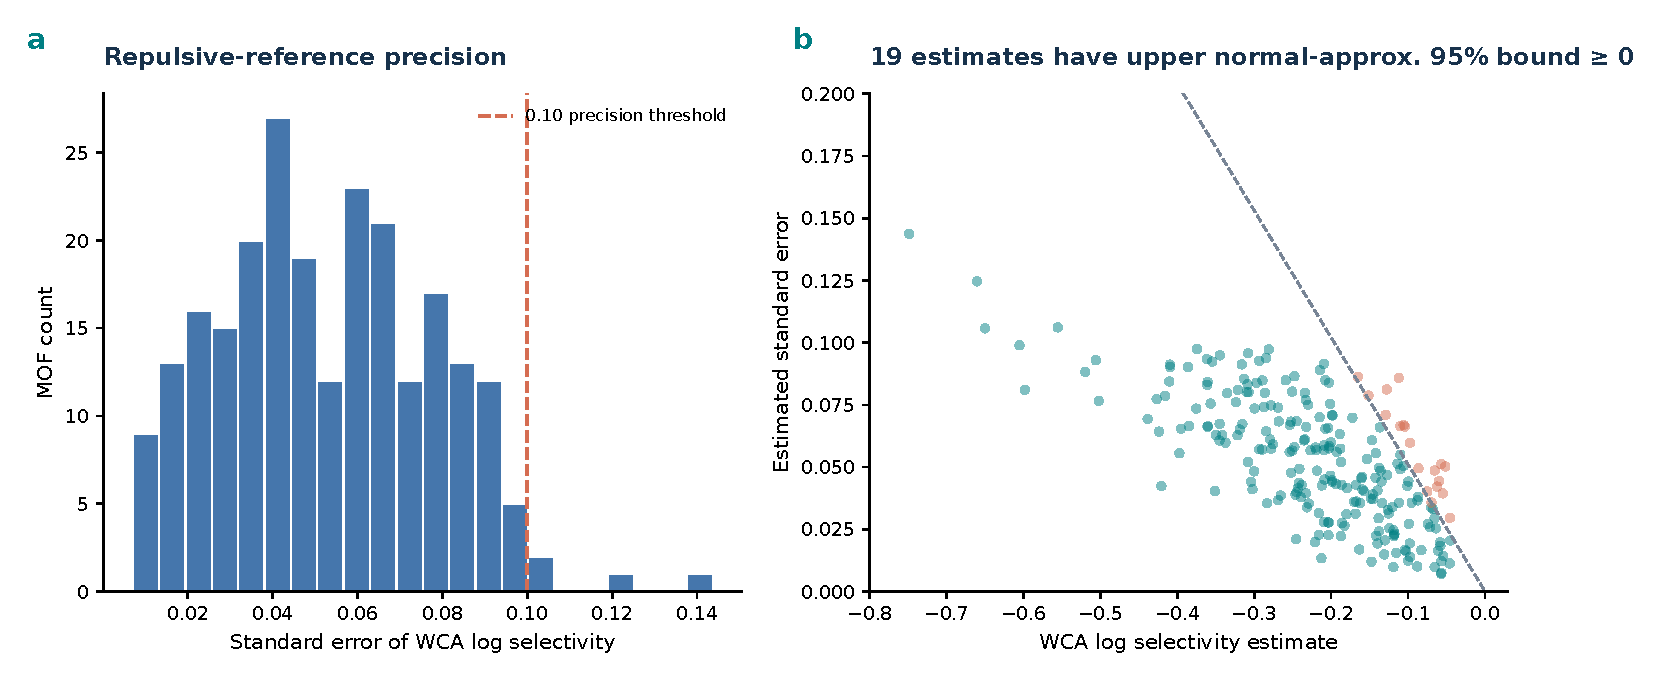
\includegraphics[width=\linewidth]{figS1_precision_diagnostics.pdf}
\caption{\textbf{Uncertainty in repulsive-reference selectivity.} (a) Distribution of the framework-level reported $\mathrm{SE}(\ln S_{\rm WCA})$. (b) Estimated WCA log-selectivity against its standard error. Nineteen individual intervals have an upper normal-approximation 95\% limit at or above zero, although all 238 central estimates are negative. The dashed boundary indicates $\ln S +1.96\,\mathrm{SE}=0$. These are approximate intervals, not a replacement for recalculation from raw seed-level insertion series.}
\label{fig:si_precision}
\end{figure}

\section{Exclusion sensitivity}

\begin{table}[H]
\centering
\caption{Sensitivity of the mechanism summaries to predefined exclusions.}
\begin{tabular}{lrrrrr}
\toprule
Population & $n$ & med. $\ln S_{\rm WCA}$ & med. $\Delta\ln S_{\rm attr}$ & med. $\Delta\ln S_{\rm elec}$ & $\rho_{\rm attr,elec}$\\
\midrule
All & 238 & -0.204 & 2.537 & 0.309 & -0.089\\
Precision pass & 234 & -0.203 & 2.510 & 0.309 & -0.094\\
Exclude top 1\% WCA & 235 & -0.207 & 2.551 & 0.309 & -0.082\\
Exclude top 1\% attraction & 235 & -0.203 & 2.510 & 0.309 & -0.091\\
Exclude top 1\% electrostatics & 235 & -0.204 & 2.542 & 0.308 & -0.087\\
Exclude top 1\% full selectivity & 235 & -0.203 & 2.510 & 0.308 & -0.117\\
\bottomrule
\end{tabular}
\end{table}

In every listed population, the WCA-positive fraction remains zero while the attractive- and electrostatic-positive fractions remain one.

\section{Geometry-only models}

The final information-content analysis used 14 pre-simulation geometry descriptors. ExtraTrees regressors contained 500 trees, minimum leaf size three, and maximum-feature fraction 0.7. Five-fold shuffled cross-validation used random seed 20260918.

\begin{table}[H]
\centering
\caption{Five-fold cross-validated geometry-only prediction. The reference MAE is the error of the full-cohort target median, not an out-of-fold fitted baseline.}
\begin{tabular}{lrrr}
\toprule
Target & $R^2$ & MAE & Baseline MAE\\
\midrule
$\ln S_{\rm WCA}$ & 0.835 & 0.033 & 0.093\\
$\Delta\ln S_{\rm attr}$ & 0.874 & 0.177 & 0.549\\
$\Delta\ln S_{\rm elec}$ & 0.188 & 0.146 & 0.147\\
$\ln S_{\rm full}$ & 0.845 & 0.189 & 0.501\\
\bottomrule
\end{tabular}
\end{table}

The restored 14-feature manifest contains only the pre-simulation geometry columns; the archived pipeline excludes target-derived adsorption quantities and identifiers. Median imputation and standardization are inside the training-fold pipeline according to the inspected source. The saved geometry OOF table has 952 rows (238 frameworks for four targets) and reproduces the reported scores without refitting. Fold membership is reconstructed from the archived KFold protocol, seed 20260918 and unchanged source row order; it was not independently saved as a historical fold file. The full-cohort median is used only as a descriptive reference for the MAE ratio. Source code inspection and saved-prediction arithmetic do not constitute a fresh training replay.

\section{Geometry-matched pairs}

The original illustrative selector uses each framework's three nearest neighbors in the standardized nine-descriptor space, retains only source-row pairs with $i<j$, and keeps the lower distance quartile of the resulting 384 candidates. Maximizing the coordinate contrast within those 96 candidates yields the retained examples below. This row-order-dependent candidate construction differs from an exhaustive all-pair search. We preserve its examples and separately enumerate the closest 2\% of all 28,203 pairs (564 candidates) in the reconciled analysis. The original code establishes the implemented operation, not an independently verified preregistration date.

\begin{table}[H]
\centering
\caption{Geometry-matched case studies.}
\begin{tabular}{lrrrr}
\toprule
MOF & $\ln S_{\rm WCA}$ & $\Delta\ln S_{\rm attr}$ & $\Delta\ln S_{\rm elec}$ & $\ln S_{\rm full}$\\
\midrule
M089 & -0.321 & 2.626 & 0.466 & 2.770\\
M192 & -0.248 & 3.283 & 0.140 & 3.175\\
M029 & -0.201 & 2.839 & 0.141 & 2.779\\
M085 & -0.198 & 2.211 & 2.001 & 4.014\\
\bottomrule
\end{tabular}
\end{table}

The all-pair optima are distinct from the illustrative cases: M099/M136 maximizes attraction contrast within the 564-pair set (geometry distance 0.463; attraction contrast 1.367), and M043/M085 maximizes electrostatic contrast (distance 0.395; electrostatic contrast 1.892). Their full identifiers, candidate sets, exact values and original alias mapping are released in the pair-selection reconciliation tables. The retained M089/M192 and M029/M085 figures and scalar values are unchanged and are not presented as these exhaustive optima.

M089/M192 have standardized geometry distance 0.199; M192 is the nearest geometry neighbor of M089 and M089 is the third-nearest neighbor of M192. Their attractive increments differ by 0.658.

M029/M085 have standardized geometry distance 0.258 and are mutual nearest neighbors. Their electrostatic increments differ by 1.860. The attraction pair is retained as a scalar case study only; its available LJ spatial maps cannot isolate the attractive increment because WCA spatial fields were not calculated.

\section{Gas-resolved electrostatic increments and limitations of archived spatial maps}

The complete 238-material result table contains full and LJ-only log Henry coefficients for both CO$_2$ and N$_2$. These make it possible to calculate gas-specific effects directly, without reconstructing a spatial field:
\begin{align}
\Delta_g\ln K_H =\ln K^{\rm full}_{H,g}-\ln K^{\rm LJ}_{H,g},\qquad
\Delta\ln S_{\rm elec}=\Delta_{\mathrm{CO_2}}\ln K_H-\Delta_{\mathrm{N_2}}\ln K_H.
\end{align}
The resulting distributions and pairwise CO$_2$/N$_2$ responses are shown in Figure~\ref{fig:si_gas}. The analysis should not assume that the finite difference isolates an experimentally measurable electrostatic free energy. It is a switch-on difference under the defined potential pathway.

\begin{figure}[tbp]
\centering
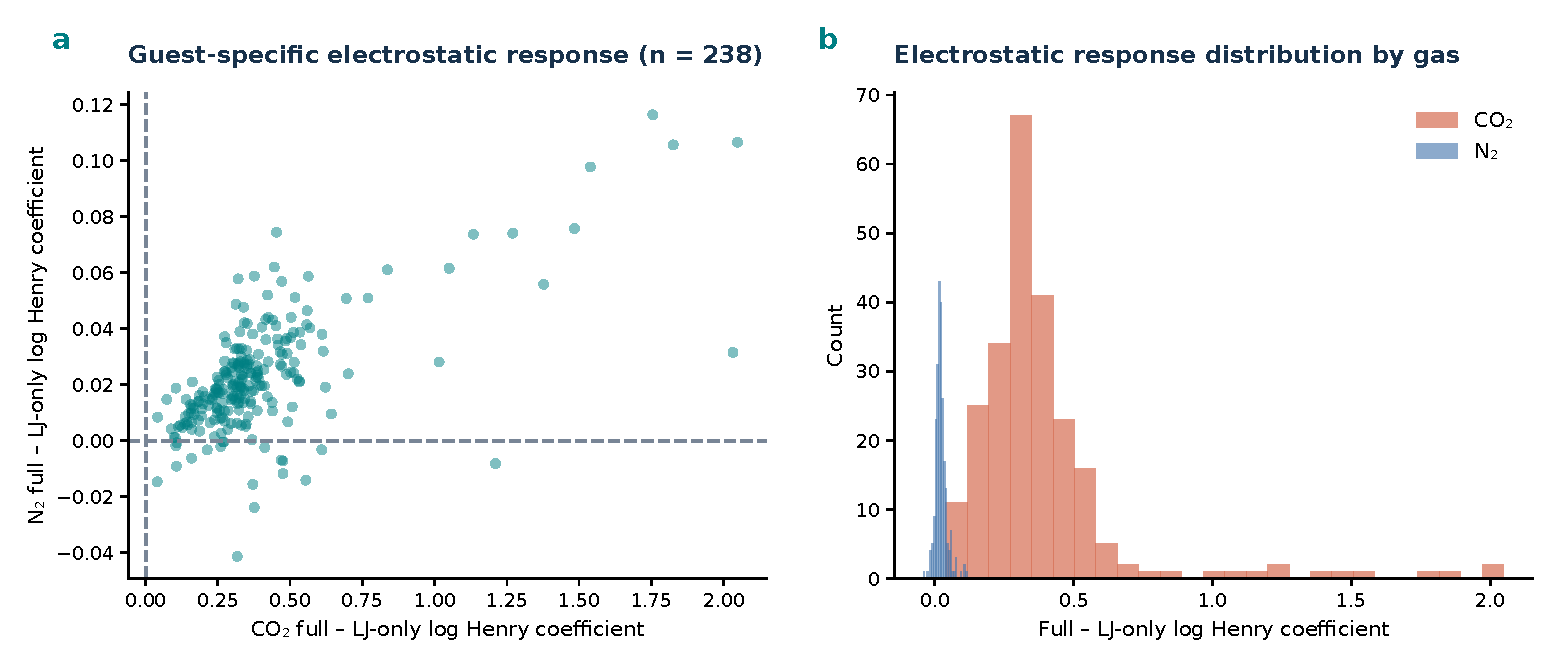
\includegraphics[width=\linewidth]{figS2_gas_specific_increment.pdf}
\caption{\textbf{Guest-specific changes upon restoring electrostatics.} (a) Framework-level CO$_2$ and N$_2$ full-minus-LJ log-Henry changes, computed directly from the authoritative production summary. (b) Distributions of the two gas-specific increments. A positive electrostatic selectivity contribution can arise from differences in two positive or negative guest-specific increments; the graph shows their actual population relationship without independently fitted spatial fields.}
\label{fig:si_gas}
\end{figure}

The earlier v5 archive includes rendered local electrostatic insertion maps and describes a $0.75$~\AA{} grid, probability-supported voxel weighting and orientation convergence tests. Those historical renderings and their spatial grids are outside this clean analytical release. The quantitative matched-pair statement relies on the verified global Henry coefficients; no new spatial field or microscopic mechanism attribution is inferred from rendered maps.

For the M029/M085 matched pair, the global CO$_2$ full-minus-LJ log-Henry increments are 0.162 and 2.032, while N$_2$ increments are 0.021 and 0.032. The between-material difference is approximately 1.871 log units for CO$_2$ but only 0.011 for N$_2$. Thus the large selectivity contrast is dominated by the CO$_2$ response in the available calculations.

\section{Additional sensitivity analyses from the archived results}

\subsection{Framework bootstrap}

Five thousand framework-level bootstrap resamples were used to quantify uncertainty in the existing-data additions. The median attractive increment is 2.537 (95\% interval 2.438--2.624), the median electrostatic increment is 0.309 (0.293--0.323), and the attractive--electrostatic Spearman correlation is $-0.089$ with a 95\% interval of $-0.222$ to 0.050. The attractive and electrostatic increments remain positive in every bootstrap resample.

For the frozen geometry-only out-of-fold predictions, $R^2_{\rm attr}=0.874$ and $R^2_{\rm elec}=0.188$, giving $G=0.686$. Resampling those frozen out-of-fold predictions gives a 95\% interval of 0.560--0.905 for $G$. This interval quantifies uncertainty in the realized out-of-fold prediction set; the model was not refitted inside each bootstrap.

\subsection{Endpoint-matched mechanism non-uniqueness}

Among all 28,203 framework pairs, the closest 5\% in final $\ln S$ were retained before mechanism distance was inspected. This gives 1,411 endpoint-matched pairs with a maximum endpoint difference of 0.0538. Their median mechanism distance is 0.189, the 95th percentile is 0.750, and the 99th percentile is 1.534. The strongest selected pair differs by 0.016 in final $\ln S$ but by 2.585 in the two-dimensional mechanism vector.

\subsection{Additional leverage sensitivity}

Removing the upper 5\% of the attractive increment gives $\rho_{\rm attr,elec}=-0.092$; removing the upper 5\% of the electrostatic increment gives $-0.084$; removing the upper 5\% of final selectivity gives $-0.179$. Removing the ten largest attraction-driven rank movers gives $-0.105$, and removing the ten largest electrostatic rank movers gives $-0.083$. The weak population association is therefore not created by a few extreme frameworks.

\subsection{Geometry-conditioned shuffle diagnostic}

A secondary geometry-conditioned shuffle diagnostic was also run using deterministic balanced strata in the first two principal components of the 14 frozen geometry descriptors. The first two components explain 92.87\% of the descriptor variance. Eight-, ten-, and twelve-stratum definitions were tested, with 10,000 within-stratum shuffles for each target while the original out-of-fold prediction was held fixed.

This diagnostic did \emph{not} support the stronger hypothesis that the attraction coordinate should show a larger excess-over-geometry-null association than the electrostatic coordinate. For the primary ten-stratum analysis, observed prediction--target Spearman correlations are 0.924 for attraction and 0.293 for electrostatics, whereas the corresponding shuffle-null 97.5th percentiles are 0.894 and 0.154. The same qualitative result occurs for eight and twelve strata. We therefore do not use this diagnostic as evidence that electrostatics is independent of geometry. Its role is to bound the claim: conventional geometry predicts attraction much more strongly in absolute out-of-fold performance, but some finer-grained geometry association with the electrostatic increment remains detectable.

\subsection{Bounded electrostatic-probe pilot}

A final pre-specified Gate C test asked whether an accessible-pore electrostatic probe could provide a positive physical coordinate for the framework-to-framework variation in $\Delta\ln S_{\rm elec}$. The implementation used identical full and LJ-only poses, 16 deterministic molecular orientations per center-of-mass position, LJ-weighted position statistics, and a fixed eight-framework numerical preflight panel. The primary descriptors were weighted medians, favorable-tail quantiles, interquartile ranges, fractions with electrostatic stabilization greater than $k_{\rm B}T$, orientation-sensitivity measures, and the corresponding CO$_2$--N$_2$ contrasts.

The 3,000$\rightarrow$6,000-position preflight did not satisfy the frozen convergence threshold for all descriptors, so the one permitted 6,000$\rightarrow$10,000-position retry was performed. At 10,000 positions, only the CO$_2$ favorable-tail descriptor met the required maximum standardized change of 0.10; the remaining descriptors did not. The two physically oriented checks remained stable: the CO$_2$--N$_2$ median-gap and favorable-tail-gap orderings each had Spearman $\rho=0.976$ between 6,000 and 10,000 positions, and both retained the pre-existing direction M085 $>$ M029. Because the descriptor-level convergence gate nevertheless failed, the 238-framework production calculation and downstream geometry/probe model comparison were not run. This test is therefore retained only as a non-supporting numerical diagnostic and does not alter the manuscript claims.

\section{Population-wide rank changes}

\begin{table}[H]
\centering
\caption{Changes in candidate ordering after each interaction stage. Rank 1 denotes the highest selectivity.}
\footnotesize
\setlength{\tabcolsep}{3.8pt}
\begin{tabular}{lrrrrr}
\toprule
Transition & Spearman $\rho$ & Median $|\Delta rank|$ & $n(|\Delta rank|\geq50)$ & Max promotion & Max demotion\\
\midrule
WCA $\rightarrow$ LJ-only & -0.751 & 102 & 183 & 234 & 226\\
LJ-only $\rightarrow$ full & 0.905 & 9 & 12 & 175 & 55\\
\bottomrule
\end{tabular}
\end{table}

The attraction step therefore reorganizes the ranking throughout the population, whereas electrostatics mostly preserves the global ordering but creates a smaller number of large rank changes.

\section{WCA force-field bridge}

The 15-MOF bridge panel was selected before the alternative-force-field results were inspected. Supported linker and main-group framework atoms were reassigned from UFF to DREIDING while cobalt retained UFF. Guest models, charges, structures, and the WCA construction were unchanged.

\begin{table}[H]
\centering
\caption{WCA sensitivity to the tested DREIDING-linker/UFF-Co perturbation.}
\begin{tabular}{lrrrr}
\toprule
Gas & $n$ & MAE $|\Delta\mu^{\rm ex}|$ & Max. $|\Delta\mu^{\rm ex}|$ & Spearman $\rho$\\
 & & (kcal mol$^{-1}$) & (kcal mol$^{-1}$) & \\
\midrule
CO$_2$ & 15 & 0.0227 & 0.0563 & 0.996\\
N$_2$ & 15 & 0.0178 & 0.0507 & 1.000\\
\bottomrule
\end{tabular}
\end{table}

\noindent\textit{Data provenance note.} The reconciled release restores 90 matched seed rows and 30 framework/gas mean rows for this bridge. Its reported aggregate MAE, maximum shifts and rank correlations are independently reaggregated from those rows. This reanalysis does not rerun the alternative-force-field simulations or reproduce the legacy rendered plot.

\section{Version-specific prediction metrics and cross-validation caution}

The version-2 \texttt{figure\_3\_source.csv} file contains results for an earlier model, including electrostatic $R^2=0.032$. The final 14-feature evaluation reported $R^2=0.188$, MAE $0.146$ and full-cohort median-reference MAE $0.147$. The initial v9 ZIP contained only a transcription of those final metrics. The reconciled release restores their matching archived OOF vectors, feature manifest, fitting-protocol source and bootstrap records. Metrics and confidence intervals are recomputed from those saved vectors without fitting a model. A neighboring 25-feature descriptor analysis produces different scores and is not substituted. The earlier v2 group-holdout results remain historical sensitivity evidence with a different model specification.

The difference is important when interpreting numerical evidence. Reporting the later random-CV numbers beside earlier group-holdout numbers without qualification could imply an invalid controlled comparison. Accordingly, the main text reports the frozen version-5 numbers and describes the version-2 holdouts only qualitatively as an indication that extrapolation beyond related framework families can be difficult.


\section{Family composition, coverage and new descriptive comparisons}

The supplementary data audit uses the string prefix before the first underscore as a database-identifier family and the final underscore-delimited token as a topology suffix. These are available metadata labels and are not treated as a substitute for a structural graph or a newly validated metal coordination environment. The analysis includes 210 entries in DB0-m15 and 28 in DB0-m12, and the \texttt{fsc} suffix appears 171 times. The distinction is particularly important because a random split can put closely related structures into both training and test sets. It would be inappropriate to describe such a split as an independent family-transfer experiment.

\begin{table}[H]\centering\small
\caption{Exploratory within-family summaries computed directly from the 238-row source table. Correlations are Spearman values between attractive and electrostatic increments; the 28-member group is comparatively small.}\begin{tabular}{lrrrrr}\toprule
Identifier family & $n$ & Median $L_{\rm WCA}$ & Median $A$ & Median $E$ & $\rho(A,E)$\\\midrule
DB0-m15 & 210 & $-0.215$ & 2.599 & 0.308 & $-0.126$\\
DB0-m12 & 28 & $-0.087$ & 1.755 & 0.313 & $+0.512$\\\bottomrule\end{tabular}\end{table}

In both families the central tendencies preserve the ordering of stages observed in the full panel. The attractive median nevertheless differs appreciably, and the within-family attraction--electrostatics associations even have opposite signs. This is not proof of contrasting universal physical laws: the families differ in size and may reflect correlated chemical choices. It illustrates the cost of interpreting pooled behavior as chemically universal. An independent extension should intentionally sample metal, linker and topology diversity rather than just increasing the number of members of an already dominant family.

\begin{figure}[tbp]\centering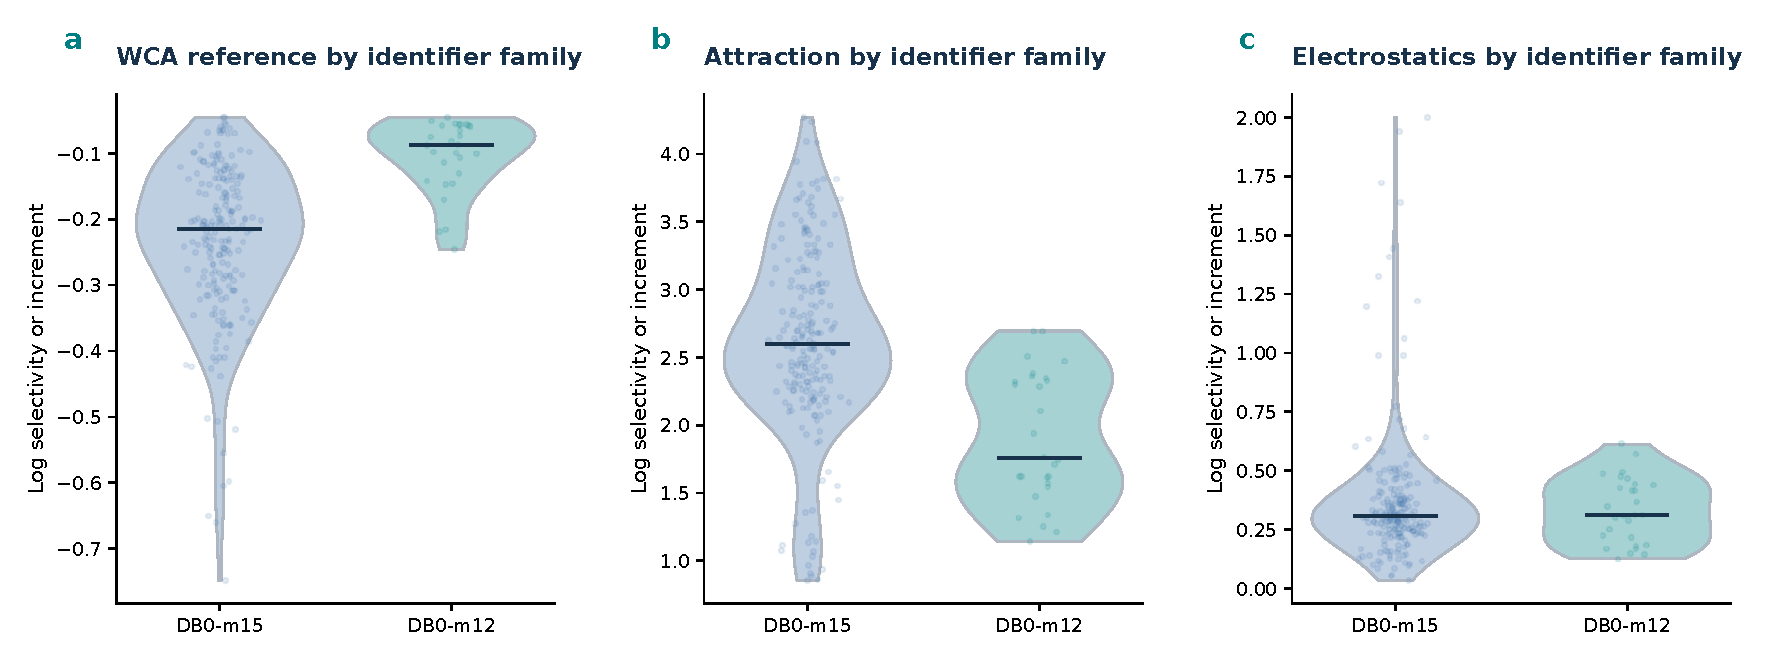
\includegraphics[width=\linewidth]{figS3_family_details.pdf}
\caption{\textbf{Family-aware exploratory diagnostics.} Distributions of (a) the WCA reference, (b) attractive increments, and (c) electrostatic increments in DB0-m15 and DB0-m12. Each observation originates in the archived authoritative table; no separate simulation is implied.}\label{fig:sifam}\end{figure}

\section{Top-list composition and its limits as a decision diagnostic}

For each state, frameworks are ranked in descending order of the corresponding log selectivity. Rank 1 means the highest predicted CO$_2$/N$_2$ Henry ratio. The shortlist length is fixed at $k=24$, close to one tenth of the 238-member population. Let $T_A(k)$ denote the set of the $k$ highest-scoring candidates in state $A$. The reported list-overlap score is $|T_A(k)\cap T_B(k)|$; it is a count, not an inferred probability of a material remaining competitive under conditions other than those simulated.

The archived data give zero common candidates between WCA and LJ-only among the top 24, and 17 common candidates between LJ-only and full. The corresponding overlap fractions are 0 and $17/24=0.7083$. In the second transition, seven entries leave and seven join the fixed-length shortlist. This statement is different from saying that 17 entries are unchanged in rank; an entry can remain shortlisted while moving several positions.

\begin{table}[H]\centering\small
\caption{Additional shortlist comparisons derived from the authoritative table.}\begin{tabular}{lrrr}\toprule
Transition & Shortlist size & Common entries & Changed members\\\midrule
WCA $\rightarrow$ LJ-only & 24 & 0 & 24\\
LJ-only $\rightarrow$ full & 24 & 17 & 7\\\bottomrule\end{tabular}\end{table}

These comparisons are exploratory and were derived after the original main analysis; they are presented as descriptive findings rather than as preregistered hypothesis tests. Shortlist overlap is sensitive to the chosen list length, ties, and near-ties. The figure-generation script uses a stable descending sort and resolves any ties deterministically by framework ID. In a more demanding study, source-level uncertainties in each Henry coefficient should be propagated through the ordering to estimate probabilities of candidate inclusion. That uncertainty-calibrated ranking exercise is not performed here.

\begin{figure}[tbp]\centering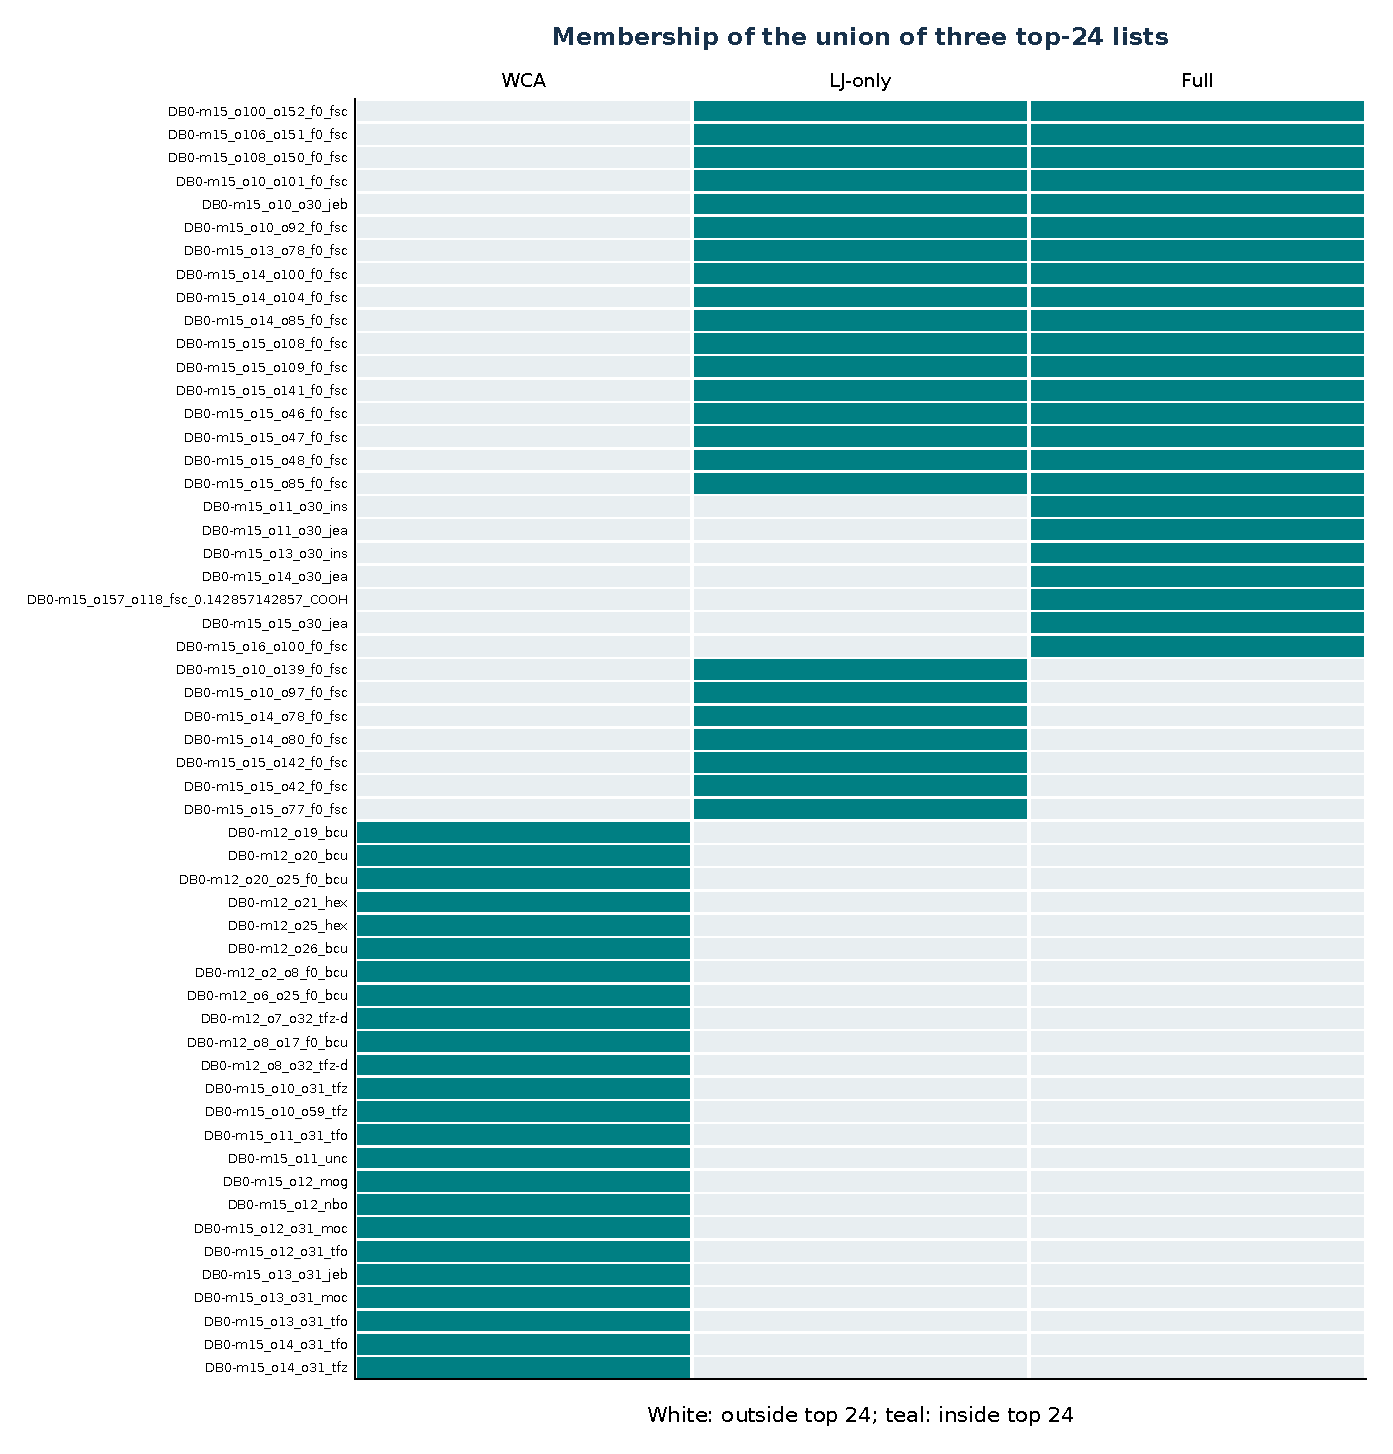
\includegraphics[width=\linewidth]{figS4_shortlist_membership.pdf}
\caption{\textbf{Membership of the 24-material shortlists.} Presence and absence of the union of shortlisted frameworks in three nested potential states; this matrix is generated from the source table rather than from graphical digitization.}\label{fig:sitop}\end{figure}

\section{Practical instructions to reproduce the manuscript figures}

The script \texttt{scripts/regenerate\_figures.py} accepts the source CSVs and generates the five original main-data figures, the new family/shortlist main figure, the extended SI figures, and a table-of-contents graphic. It does not call RASPA or LAMMPS, download structural data, or infer missing numerical voxel fields. The companion \texttt{scripts/make\_results.py} writes the final coordinate, family, shortlist, endpoint and pair-selection reconciliation tables and exports the explicit figure inputs; all calculations use the preserved cohort and saved prediction evidence.

From the extracted package root on Windows, the core commands are:
\begin{verbatim}
python -m pip install -r requirements.txt
python scripts/make_results.py
python scripts/make_figures.py
python scripts/verify_package.py --prepare-checksums
python scripts/write_checksums.py
python scripts/verify_package.py
\end{verbatim}

The exact file names needed for analytical regeneration are documented in \texttt{README.md} and a SHA-256 manifest. For clarity, the key input files are:
\begin{verbatim}
data/authoritative/mechanism_238_authoritative.csv
data/final/geometry_oof_predictions.csv
data/final/geometry_cv_metrics.csv
data/provenance/descriptor_hierarchy_predictions.csv
data/figure_sources/
data/figure_sources/SOURCE_MAP.json
\end{verbatim}
The figure generator saves vector PDF files for placement in LaTeX and losslessly compressed TIFF and PNG images for editorial use. Font sizes, line weights and color assignments are set in one central section at the beginning of the Python file. A reproducibility check verifies that all 238 identifiers are unique, that input source tables agree with authoritative data, and that the nested increment identity closes numerically. A failure raises an explicit Python error rather than silently producing visually plausible but inconsistent figures. The output summary \texttt{quality\_control/regenerated\_metrics.json} also records central numerical quantities.

To rebuild the JCTC article, compile the manuscript source using pdfLaTeX and BibTeX from the manuscript directory. Compile this Supporting Information source separately from its own directory. The names and affiliations shown are those supplied for this manuscript; author contributions, disclosures, and repository deposition require author approval before submission.

\section{How to interpret the principal limitations}

\textbf{Simulation uncertainty versus sampling coverage.} The estimated standard error associated with a Henry coefficient describes the uncertainty of a particular simulation under its sampling protocol. It does not describe uncertainty in whether a model applies to metal centers or linkers not represented in the panel. Similarly, a nonparametric framework bootstrap measures sensitivity to resampling the observed population, not uncertainty over all possible MOF structures.

\textbf{A numerical counterfactual versus a real experimental intervention.} Switching between WCA, LJ-only and full force fields does not correspond to a laboratory operation that independently removes dispersion while holding everything else fixed. The reference stages are computational instruments. Their usefulness lies in making a consistent comparison, not in treating each one as an isolated physically observed adsorption mechanism.

\textbf{Prediction versus mechanism.} A geometry-based regression can be accurate for the sum of several correlated contributions yet poor at predicting one component. That does not show that the component is independent of geometry or that the predictor learned the correct chemistry. The distinction should motivate a held-out-family challenge using a sufficiently varied material library and frozen model decisions.

\textbf{Low-pressure thermodynamics versus process performance.} Henry selectivity does not provide mixture working capacity, competitive adsorption at elevated loading, diffusion rates, regeneration energy or hydrothermal stability. An application-driven follow-up would require all of these, as appropriate to the process, before claiming improved carbon-capture performance.

\textbf{Reproducibility tiers.} The numerical paper figures and final OOF metrics are regenerated from the supplied CSV files without refitting. Fresh molecular simulation additionally requires the complete primary CIF, input-deck and executable set; that replay is not claimed for this analytical release. We explicitly identify this gap to avoid conflating plot-level and simulation-level reproducibility.


\section{Thermodynamic meaning of the insertion averages}

At infinite dilution, the energetic response to adding a test molecule can be evaluated from an ensemble average of Boltzmann factors, provided the host structure, temperature, guest model and sampling distribution are defined consistently. In the common rigid-host idealization, the insertion integral averages $\exp[-\beta U_g(\mathbf r,\Omega)]$ over spatial positions $\mathbf r$ and orientations $\Omega$, with $\beta=1/(k_{\rm B}T)$. Normalization conventions and standard-state factors matter for absolute Henry coefficients, but the ratio of two consistently calculated coefficients is a well-defined measure of low-pressure discrimination.

The nonlinear exponential average means that rare favorable insertion geometries can contribute a great deal to the overall Henry coefficient. A local attractive site does not have to occupy a large volume to influence the result; conversely, a large pore volume does not ensure a large Henry coefficient if most insertions are energetically unfavorable. This is why a geometry-only description can correlate strongly with some adsorption outputs while missing a minority of chemically distinct local environments.

A log-selectivity is convenient because ratios turn into differences. However, the reference-potential increments still reflect the combined changes in accessible configurations and energies. The attraction increment is not numerically equal to a simple average dispersion energy difference, and the electrostatic increment is not numerically equal to an average Coulomb energy difference. In either case, the change in statistical weights is included automatically. This interpretation underpins the manuscript's emphasis on ``interaction-stage'' rather than ``separable energetic'' contributions.

The two gas-specific electrostatic responses make the algebra particularly transparent. Define $d_g=\ln K_{H,g}^{\rm full}-\ln K_{H,g}^{\rm LJ}$ for each gas. Then the electrostatic change in CO$_2$/N$_2$ log-selectivity is $E=d_{\mathrm{CO_2}}-d_{\mathrm{N_2}}$. For M029 and M085, $d_{\mathrm{CO_2}}$ equals approximately 0.162 and 2.032, respectively, whereas $d_{\mathrm{N_2}}$ equals 0.021 and 0.032. Their electrostatic-selectivity difference follows directly from subtracting these two guest-specific changes. The almost complete attribution to the CO$_2$ response is therefore based on numerical values, not on interpreting colors in a heatmap.

\section{Resampling and uncertainty: what the intervals mean}

The source WCA table includes an estimated standard error for each framework's log-selectivity. To provide a simple diagnostic rather than a formal simultaneous confidence band, an approximate per-framework interval can be formed as $\widehat{L}_{\rm WCA}\pm1.96\,\widehat{\rm SE}(L_{\rm WCA})$. Nineteen of the 238 resulting upper bounds are at least zero. This is enough to disallow the statement that \emph{every individual} structure has a 95\%-resolved negative WCA log-selectivity; it does not weaken the observation that all point estimates are negative. Multiple testing and any shared simulation error would require further consideration if the purpose were formal individual discovery calls.

The framework-bootstrap interval reported in the earlier archive operates at a different level. It draws frameworks with replacement and recalculates the median or correlation on each synthetic sample. It thus describes sampling variability conditional on the observed population composition. It is not a simulation-seed bootstrap, does not replace uncertainties in the input molecular potentials, and does not simulate the probability of drawing an unrelated MOF chemistry from the world's known structures. The two types of uncertainty must not be interchanged in the presentation.

A third form of uncertainty concerns the fitted geometry controls. The initial v9 ZIP retained the final cross-validation summary as a transcription. The reconciled release restores the matching archived geometry OOF vectors and the 14-feature manifest and recomputes their metrics and bootstrap intervals. Fold metadata are reconstructed from the archived KFold seed and unchanged input ordering; the inspected source places preprocessing inside the training folds. Saved estimators were not restored and no model fit was rerun. The earlier version-2 model and the neighboring 25-feature analysis remain distinct from this final 14-feature evidence.

\section{Why the two family-specific correlations should not be overinterpreted}

The 210-entry DB0-m15 group has an attraction--electrostatics Spearman coefficient of about $-0.126$, whereas the 28-entry DB0-m12 group has a positive coefficient of about $+0.512$. These observations are useful because they show that a single pooled correlation is not the only defensible description of this concentrated data set. They do not establish two distinct chemical laws, however, because the group labels are observational and the smaller group can be disproportionately influenced by its composition and a handful of points.

The main source of difficulty is dependence between the nominal explanatory dimensions. Metal identity, topology, pore size and chemical decoration may vary together, so a model can appear accurate without isolating which variable accounts for the effect. Group-specific analysis makes the confounding visible, but breaking it requires an independent experiment or simulation design. A stronger follow-up would deliberately match geometric properties while varying a clearly characterized local chemical feature across different metals and linkers, and would measure the response under more than one charge model.

It is also important not to promote the dataset identifier suffixes into structural claims that have not been checked. In the supplied table, the family prefix and topology suffix are useful organizational metadata. The package does not contain the original CIF coordinates to independently validate atom connectivity or topology. For that reason, the current paper reports ``identifier family'' and ``topology suffix'' whenever a count comes exclusively from these strings. More chemically specific attribution must await the complete structures and a reproducible bonding analysis.

\section{A minimal independent-review test suite}

A reviewer who has extracted the ZIP can reproduce the essential plot-level claims without restarting costly Monte Carlo calculations. The first check is that the authoritative CSV has 238 distinct framework identifiers, no missing values in the three coordinates and a telescoping residual at floating-point precision. The next checks confirm that each WCA point estimate is negative, the LJ-only and full selectivities are positive, and that the medians and Spearman correlations match those stated in the Results. A further check ranks frameworks by each state and verifies the two shortlist overlaps. Finally, the regenerated figure files can be compared against the included published PDF images, without accepting a figure that was generated from hidden or unavailable data.

This is deliberately a \emph{plot-level reproducibility} test suite. It supports verification of every new descriptive result in version 9 and guards against unnoticed changes in plotting scripts or table filters. It is not sufficient to audit the microscopic force-field choices or repeat the Widom integrations. Complete simulation-level reproduction additionally requires complete structural inputs, executable versions, model parameters, seed lists and run-level outputs.


\section{Source data and reproducibility}

The reconciled release includes the unchanged authoritative 238-MOF mechanism table, archived gas-specific seed summaries, matching final 14-feature geometry OOF predictions, descriptor manifest and source protocol, bootstrap and sensitivity records, explicit figure-source tables, plotting and verification code, final documents and checksums. The earlier version-2 figure-3 data and neighboring 25-feature model are not substituted for the final scores. The recorded molecular protocol and guest/force-field definitions are supplied for provenance, but the release does not provide a complete runnable set of all original CIFs, per-job decks, executable environments or spatial voxel fields. Analytical regeneration is therefore supported; a fresh simulation or model-training replay is not claimed.

\bibliographystyle{unsrt}
\bibliography{../manuscript/references}
\end{document}
